%
% File acl2014.tex
%
% Contact: giovanni.colavizza@epfl.ch
%%
%% Based on the style files for ACL-2013, which were, in turn,
%% Based on the style files for ACL-2012, which were, in turn,
%% based on the style files for ACL-2011, which were, in turn, 
%% based on the style files for ACL-2010, which were, in turn, 
%% based on the style files for ACL-IJCNLP-2009, which were, in turn,
%% based on the style files for EACL-2009 and IJCNLP-2008...

%% Based on the style files for EACL 2006 by 
%%e.agirre@ehu.es or Sergi.Balari@uab.es
%% and that of ACL 08 by Joakim Nivre and Noah Smith

\documentclass[11pt]{article}
\usepackage{acl2014}
\usepackage{times}
\usepackage{url}
\usepackage{latexsym}
\usepackage{graphicx}
%\setlength\titlebox{5cm}

% You can expand the titlebox if you need extra space
% to show all the authors. Please do not make the titlebox
% smaller than 5cm (the original size); we will check this
% in the camera-ready version and ask you to change it back.


\title{Environment news in the world: \\ A GDELT Case Study}

\author{Damien Martin \\
  {\tt } \\\And
  Karthigan Sinnathamby \\
  {\tt EPFL Lausanne, Switzerland } \\\And
Mathieu Ducroux \\
{\tt } \\}

\date{}

\begin{document}
\maketitle

\begin{abstract}
   We conduct a study on news media coverage of environmental events through the use of the Global Database of Events, Language and Tone (GDELT). We identify the most influential actors and their interaction through a network analysis. Then, we characterize the evolution in time of two important dimensions, article quantity and sentiment, before identifying the major events related to environment. Lastly, we focus on European countries through a more spatial approach. In particular, we study whether there is a possible link between this coverage and the economy of a country. We also study the news coverage from a flip point view (how a country relates worldwide news, and how the world relates news about the country).

\end{abstract}

\section{Introduction}
The news media have become nowadays the most important source of information about world events. Undeniably, media coverage of topics influences how these topics are perceived in the society. Indeed, the news conveys not only facts but also biases through article sentiment and word selection, influencing what we think about and how.

In the last decades, environment issues have taken an important place on the world stage. Our view on environment has changed and environment related events are more put forward in our daily life. This is undeniably due in part to the extensive news coverage of these events.

In this context, we conduct a study on news media coverage of environment related events for the time period from February $18^{th}$ 2015 to November 23$^{rd}$ 2017. The goal of this study is to characterize the environment media discourse by identifying the main features that define it. For this purpose, we use the Global Database of Events, Language and Tone (GDELT) that contains news articles around the world. 

In this report, we will first explain how we use GDELT in our study. Then we will explain the results of our study that proceeds in three main phases. 
In a first phase, we want to find the major actors involved in environment-related events and how they are linked all together. 
In a second phase, we explore the media discourse from a temporal approach along two important dimensions: article quantity and sentiment of news reports. This enables us to identify several major events related to environment. 
Finally, we take a more spatial approach on the news coverage. In particular, we focus on European countries and study the spatio-temporal coverage of events happening in these countries. Then, we explore any possible relationship between these dimensions and the economy of these countries. However all the previous analysis talk about how a specific country is mentioned in the world. Therefore, we have also compared this approach to how much a specific country talks about the environment, in other words "countries mentioned by the media" vs "countries hosting the media".

\emph{We invite the reader to take a look at the appendix at the end of this report to have the plots at a better scale.}

\section{GDELT database}
The GDELT database monitors and analyses web, prints and broadcasts news around the world. We have here a massive inventory of events that is updated on a daily basis, every fifteen minutes. 

\subsection{General Appreciation}
Each news report monitored by GDELT is first processed through powerful algorithms that extract meta-data in several categories. We have used in our research the following information: Themes, Actor, Location, TimeDate, Tone.
\subsection{GDELT Filtering}

The GKG dataset contains 261'887'856 records.
We need to filter this massive database on environment related events. The V1Themes column is sorted on the order of appearance of themes in the article. In our case, if an article talks about an environment related issue, then for sure there will be an environment theme among the first themes of V1Themes. Therefore, to filter out the GDELT database, we have considered only the first five themes of this column. 
After filtering, the GKG dataset contains 9'878'377 environment related records.

\section{Influential actors}
Firstly, we study the important actors in the global media environment conversation and how they are related to each other.

\subsection{Identifying major actors}
\label{WordCloud}
We build a Word Cloud of each type of actor in the Figure \ref{actors}. This put forward the major actors that have taken part in the environment discourse on the world stage. Among the most cited persons are politicians (mostly American ones) but also storms, oceans and influential businessmen. The organization Word Cloud is dominated by the media. Associated Press is the main one, implying that most of the articles retrieved by GDELT comes from this news agency. We have also a lot of mention of environmental organizations. The country Word Cloud not only contains major countries but also smaller ones which are prone to natural disasters.

\begin{figure}
   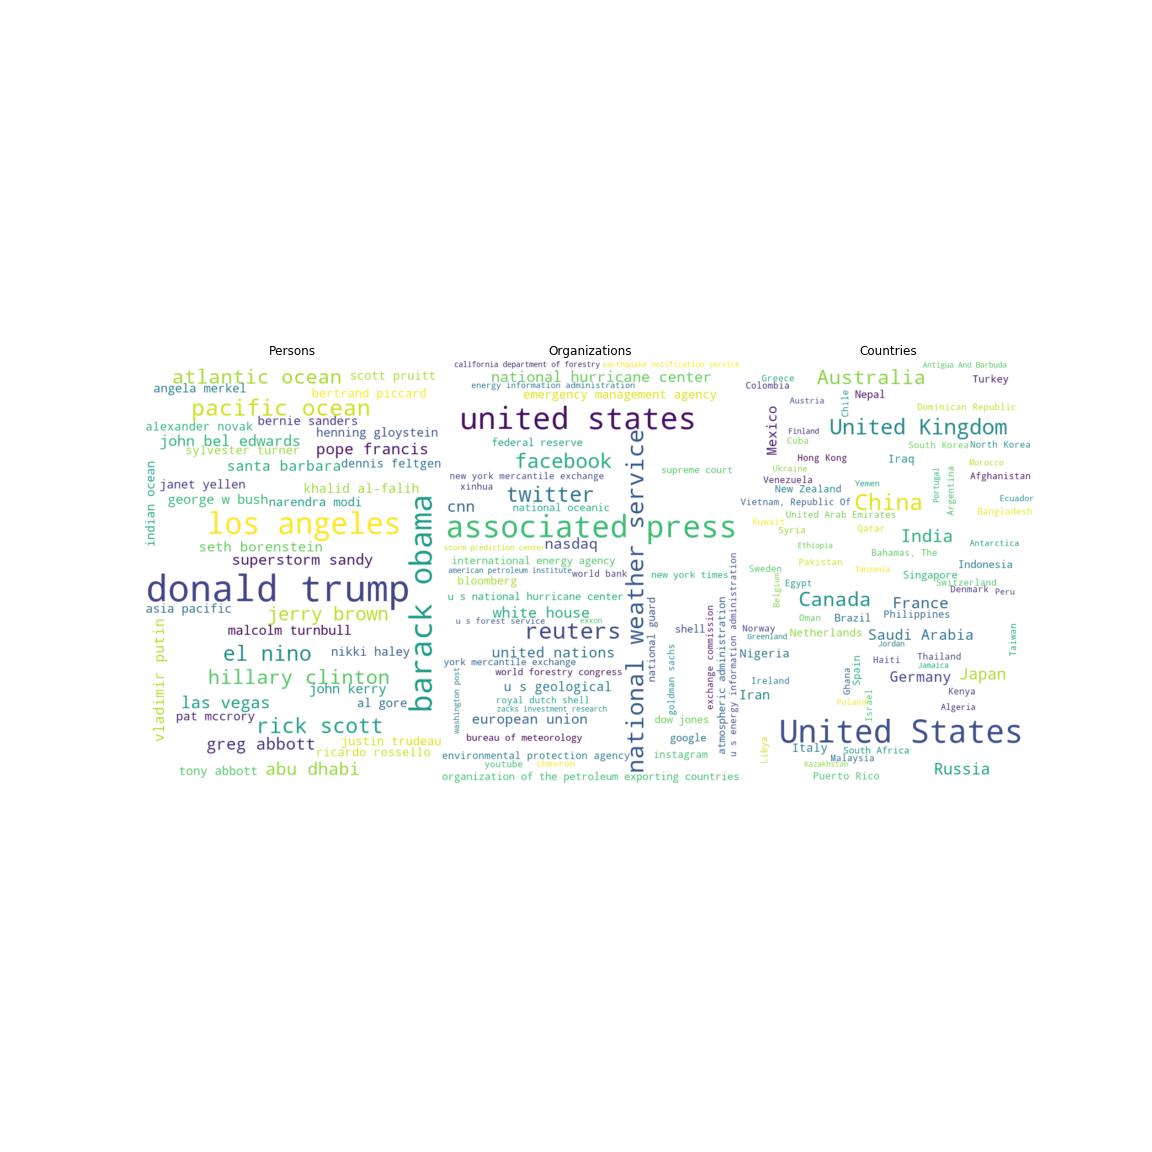
\includegraphics[scale=0.25]{wordcloud_global.png}
    \caption{\label{actors} Word Cloud of most mentioned persons, organizations and countries.}
\end{figure}

\subsection{Co-occurrence network of actors}
In order to study the links between actors, we draw a co-occurrence network (Figure \ref{network}) of the 25 most cited persons and organizations. The width of an edge is proportional to the number of times two actors appear together in an article. The size of a node is proportional to the occurrence of an actor. We use the Louvain Method for detecting communities and draw them using different colors. The graph is connected and has a high density value of 0.92. The longest shortest path is 2. This means that a lot of pairs of actors have been cited together at least once. Associated Press, the United States and Donald Trump are by far the actors with the biggest weighted degree, meaning that they appear a lot with other top actors. Finally, we can identify interesting groups of actors. In pink we have big web companies that mediate a lot of information. Oil and energy related actors are in red. In green are the American actors acting at national level while international actors are in yellow. Finally oceans and related organizations are in dark blue.

\begin{figure}
   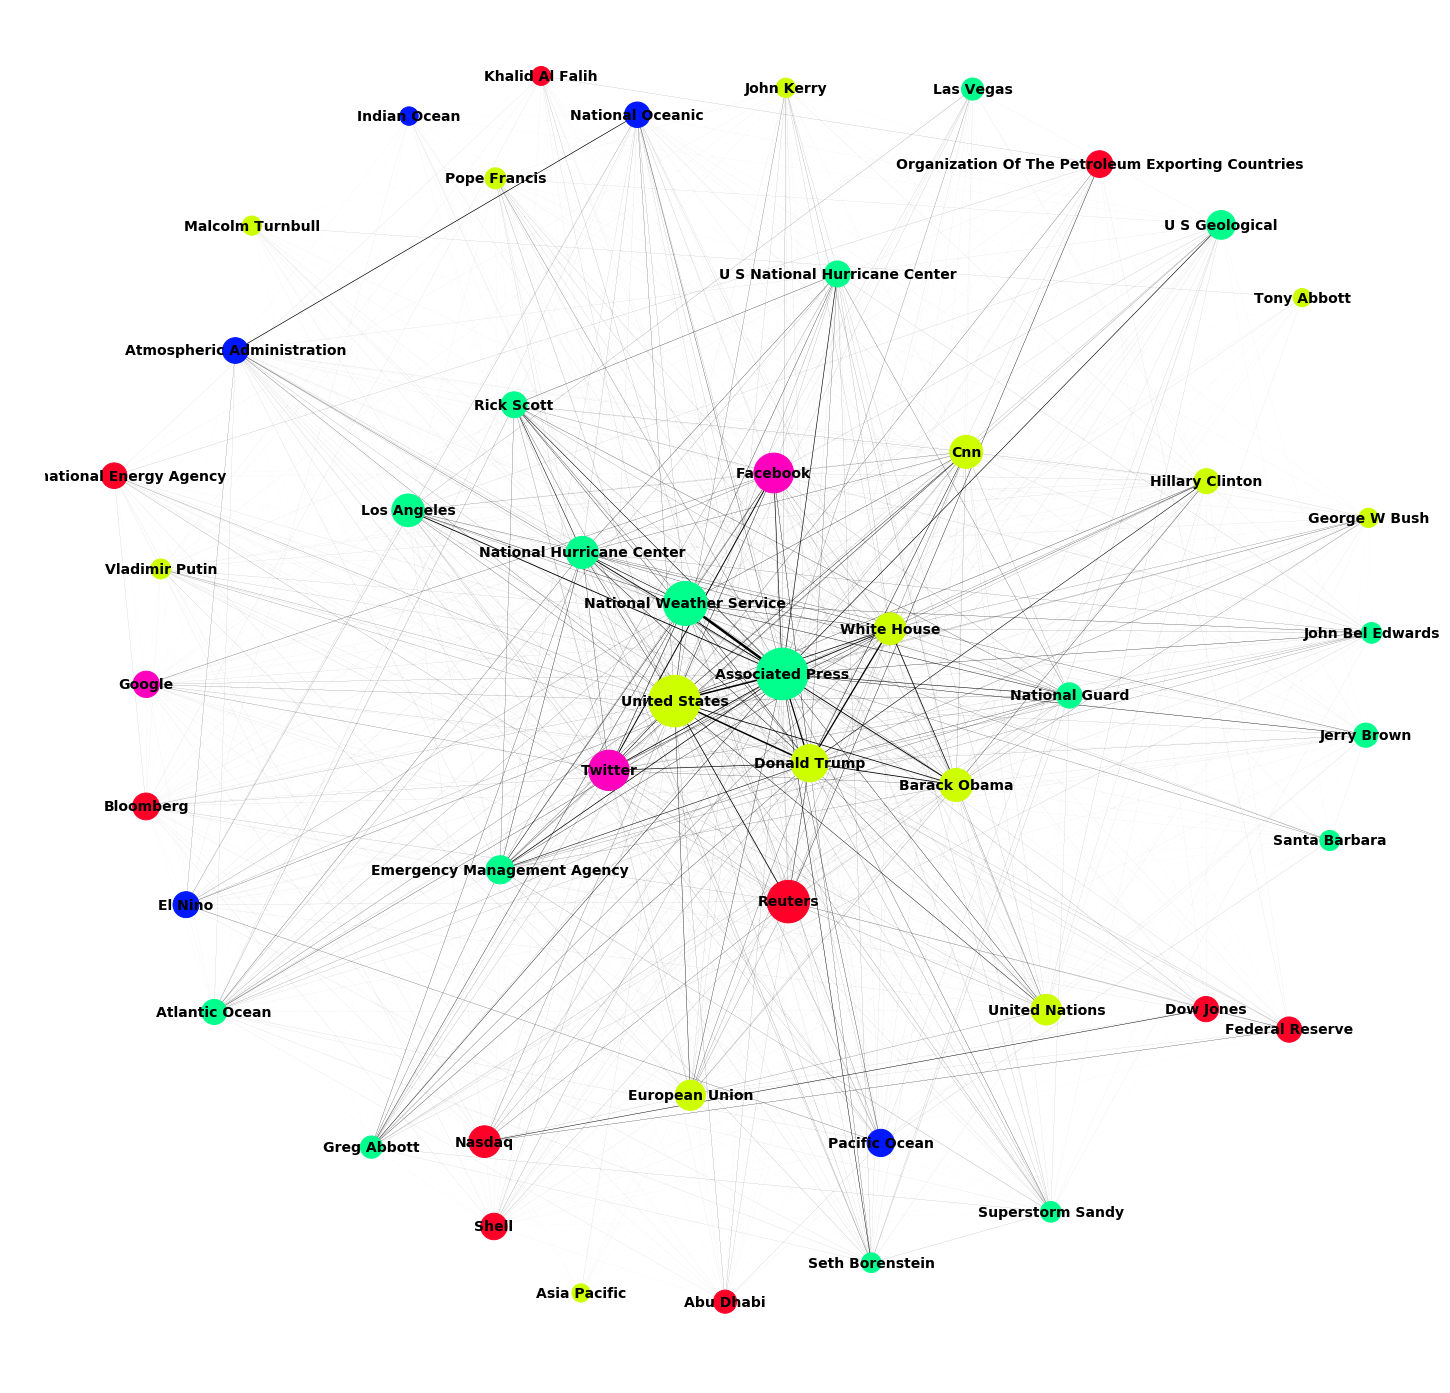
\includegraphics[scale=0.15]{top_25.png}
    \caption{\label{network} Co-occurrence network of the top 25 organizations and top 25 persons}
\end{figure}

\section{Temporal approach}
In the following, we study the media coverage from a temporal approach. That is we aim to visualize the time evolution of the sentiment of news (i.e. the tone) and the ratio of the number of environment related mentions over all mentions. From this analysis, we can further pinpoint several events that have attracted the news worldwide.

\subsection{Time evolution}
Along with the number of articles, the tone carried in news reports, whether neutral, negative or positive, has a potential impact on opinion. 
According to Figure \ref{time_evolu}, the worldwide ratio of mentions remains relatively constant throughout the three years. What is more important here is the few peaks that we can clearly distinguish on the curve. These surely correspond to particular events which have attracted the attention of the world scene.
On the same figure, we can see that the daily median tone is around -2. The negative value is predictable as environment related events are most often related to bad events inducing negative reaction from the public. The evolution in time of the tone exhibits also several peaks. We can see here, that some peaks are common between the tone and the mentions graphs, but more importantly some are not. This means that the analysis in time of both dimensions are complementary to highlight the news coverage. 

\begin{figure}
   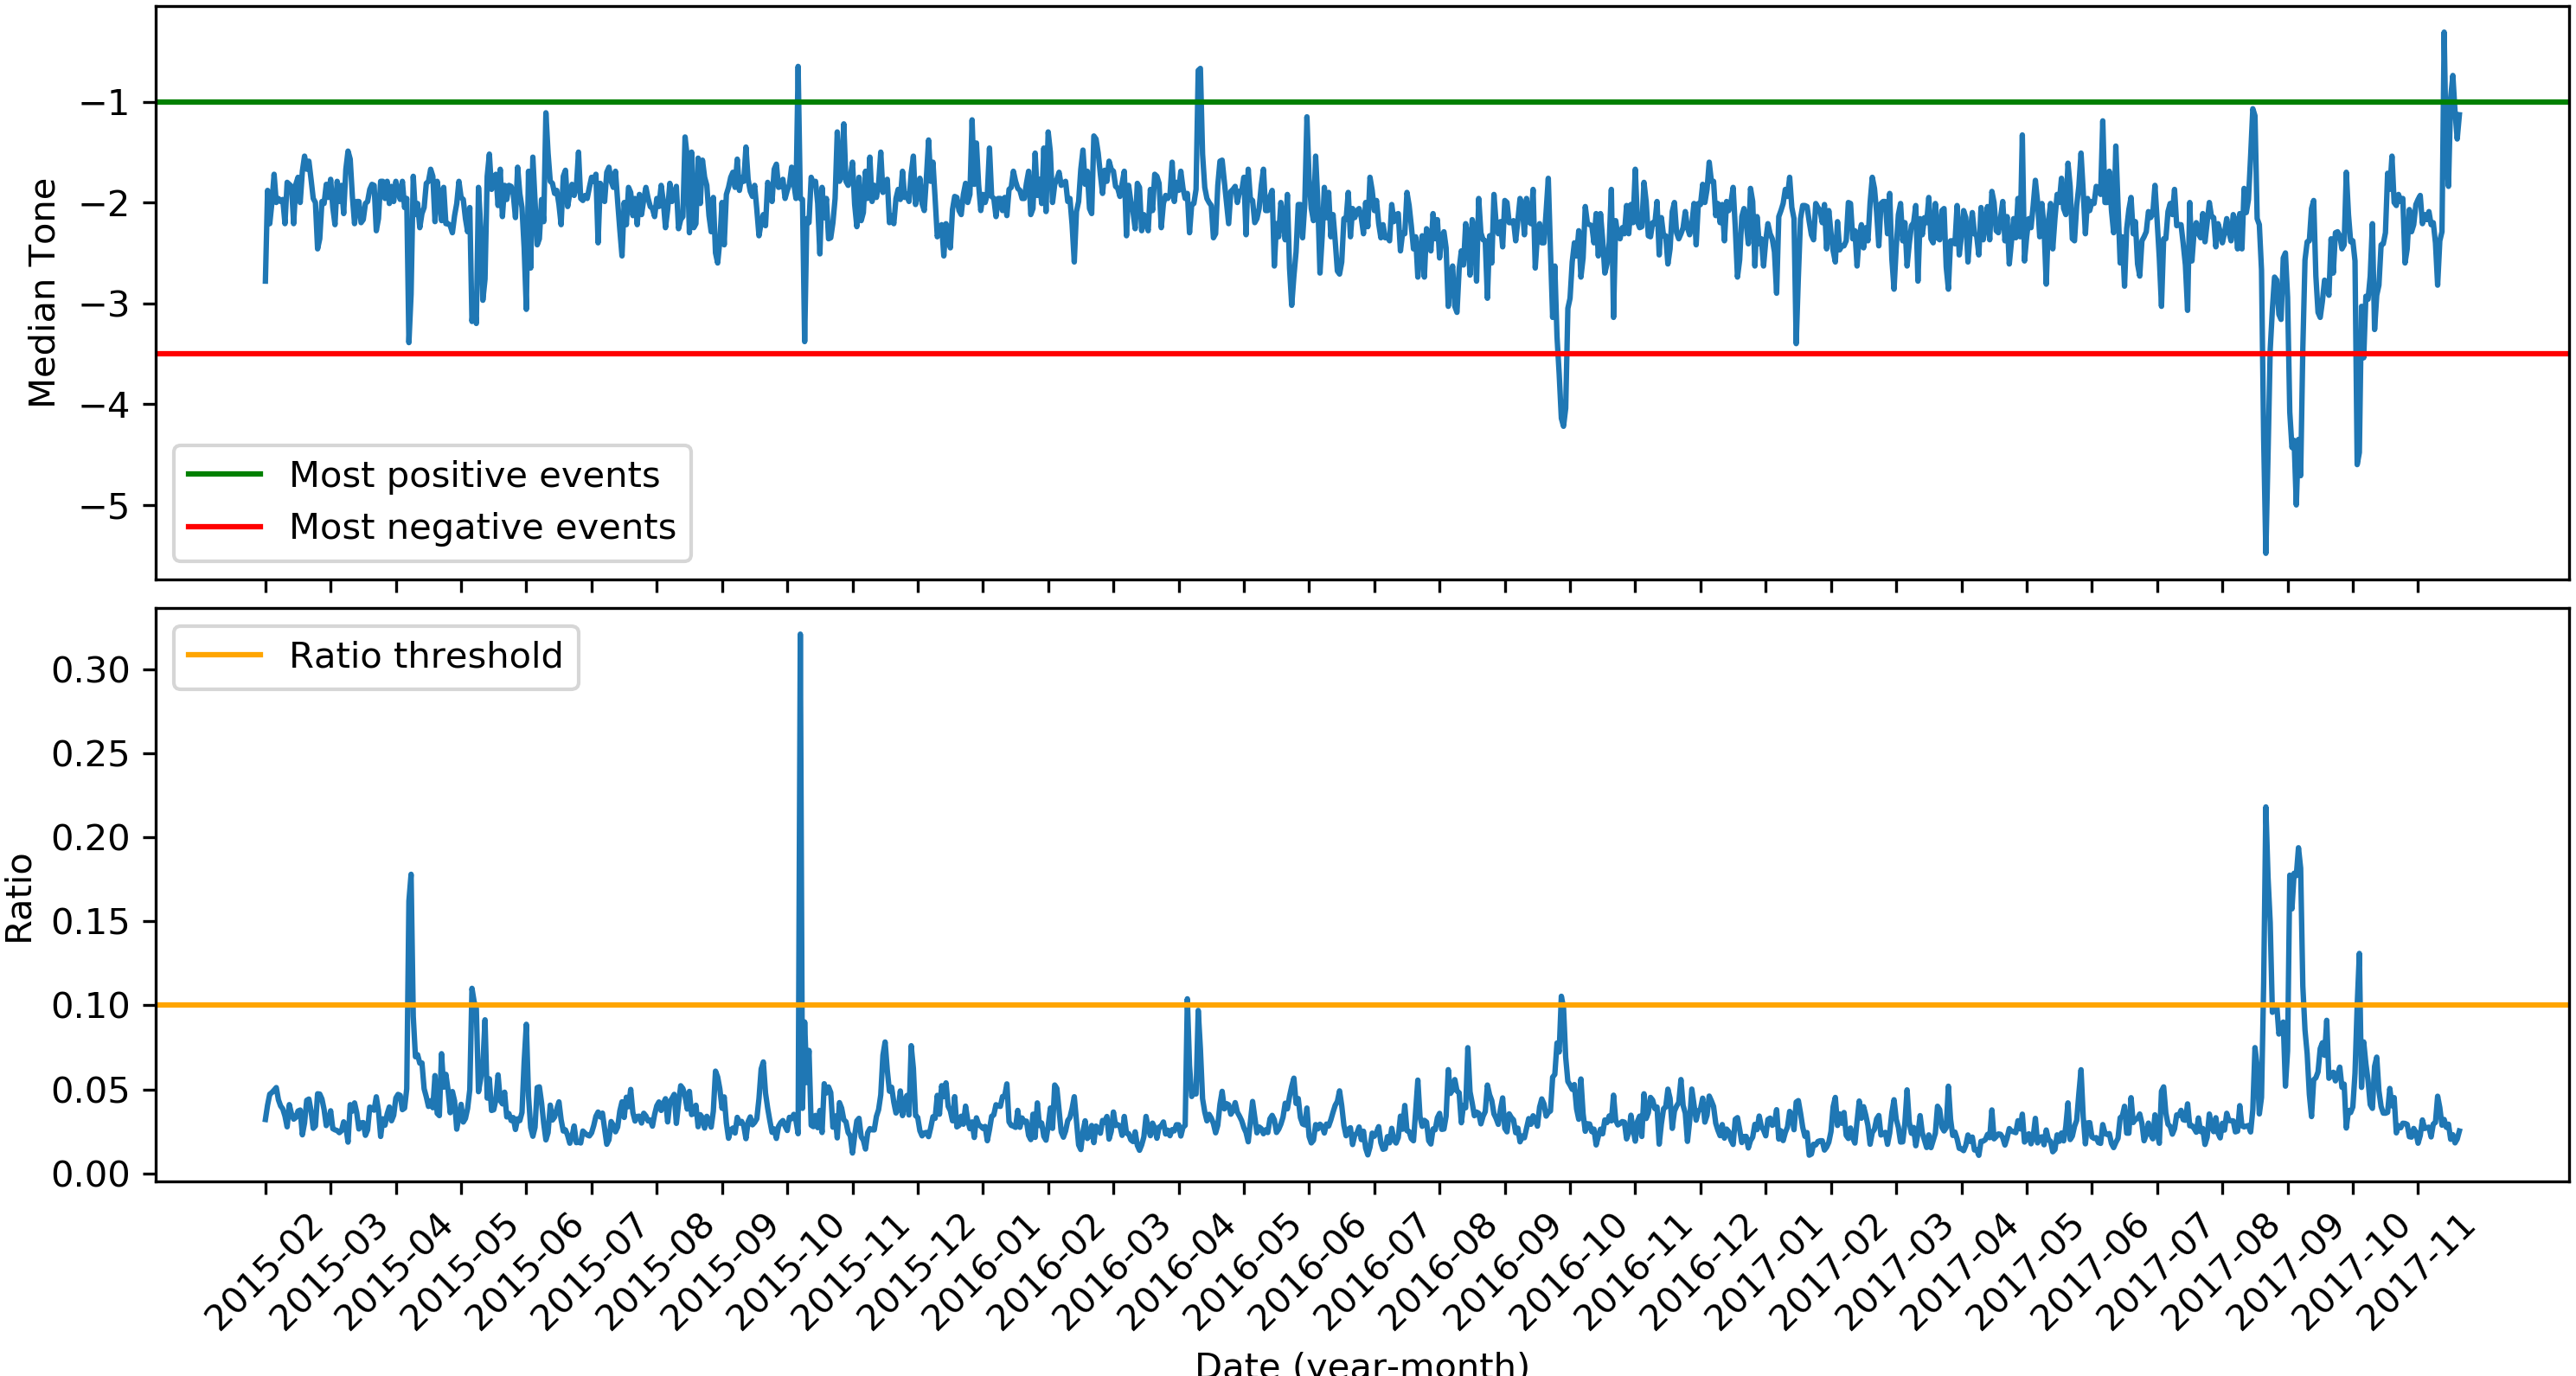
\includegraphics[scale=0.3]{global_ratio_tone_plot.png}
    \caption{\label{time_evolu} Global median tone (top) and ratio of mentions (bottom) over time (day precision). The color lines highlight the peaks corresponding to big events.}
\end{figure}

\subsection{Identifying major events}
\label{major_events}
In order to investigate which events triggered those peaks, we use the Word Cloud that we described in \ref{WordCloud}. This enables us to pinpoint the major events related to environment that have brought about a high reaction from the news media. 

We give here the analysis of the most distinguishable peak around 22/10/2015. 
The Word Cloud gives "Justin Trudeau" and "Pacific Ocean" for the persons cloud and "Puerto vallarta" for the cities cloud.

By searching for Justin Trudeau, we can find that this was the date when he was elected as the prime minister of the Canada and one theme of his campaign was to reduce the green gases emission. This corresponds to the positive shift in the tone.

From the "Pacific Ocean" and "Puerto Vallarta", we can identify that the Hurricane Particia hits Mexico on the 23/10/2015 which correspond to the negative shift in the tone.

Here, we see that the sentiment analysis gives a better appreciation of the news coverage. While the ratio of mentions put forward that there was a big event, it did not show that there were actually two big events very close in time.

\section{Spatial approach: European countries}
The overall analysis of the media coverage described in the previous section, was performed at the aggregate level across all countries and focused on the temporal side of the coverage. In the following, we zoom into the European perspective of environment media discourse to get a better grasp of the spatial dimension of the subject. 
In a first step, we study the spatio-temporal evolution at a country level. Then we look at a possible link between how the coverage and the economy of the country. 
Now, we need to point out that for these two steps, we analyse the countries as being mentioned by an article in the media. Indeed, GDELT locations field only indicates the locations associated to an actor mentioned in an article, not taking into account whether this article comes from the country. Therefore, in a final part, we compare the previous approach to the flip point view, that is with countries which the article is from.

\subsection{Spatio-temporal coverage}

\begin{figure}[h]
   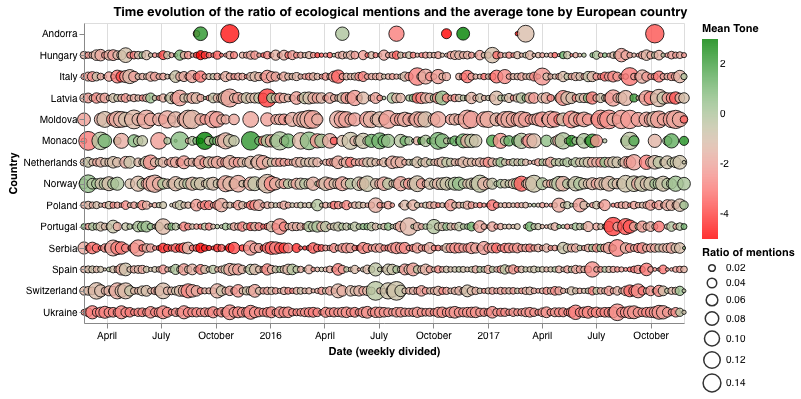
\includegraphics[scale=0.3]{timeline_europe_for_report.png}
    \caption{\label{timeline} Time evolution of the ratio of mentions and tone of articles mentioning an European country - Random Sample of 14 countries for space issue}
\end{figure}

According to Figure \ref{timeline}, we can note the heterogeneity in visibility for European countries over time in the ratio of mentions and of the tone in Europe countries. Some countries like Ukraine are continuously highly cited with a high negative tone; others like Monaco are highly cited but in a positive manner. Countries like Poland or even Andorra are less continuously cited. Overall, this bubble timeline plot shows how the European countries are cited by the entire world media (including the country itself) when it comes to environment related articles in terms of sentiment and of number of mentions. 

\subsection{Link with the economy}
We study the potential link between how a European country is mentioned regarding environment events and its economy. We rely our study on the Human development index (HDI) and on the Environment performance index (EPI).
\begin{figure}[h]
   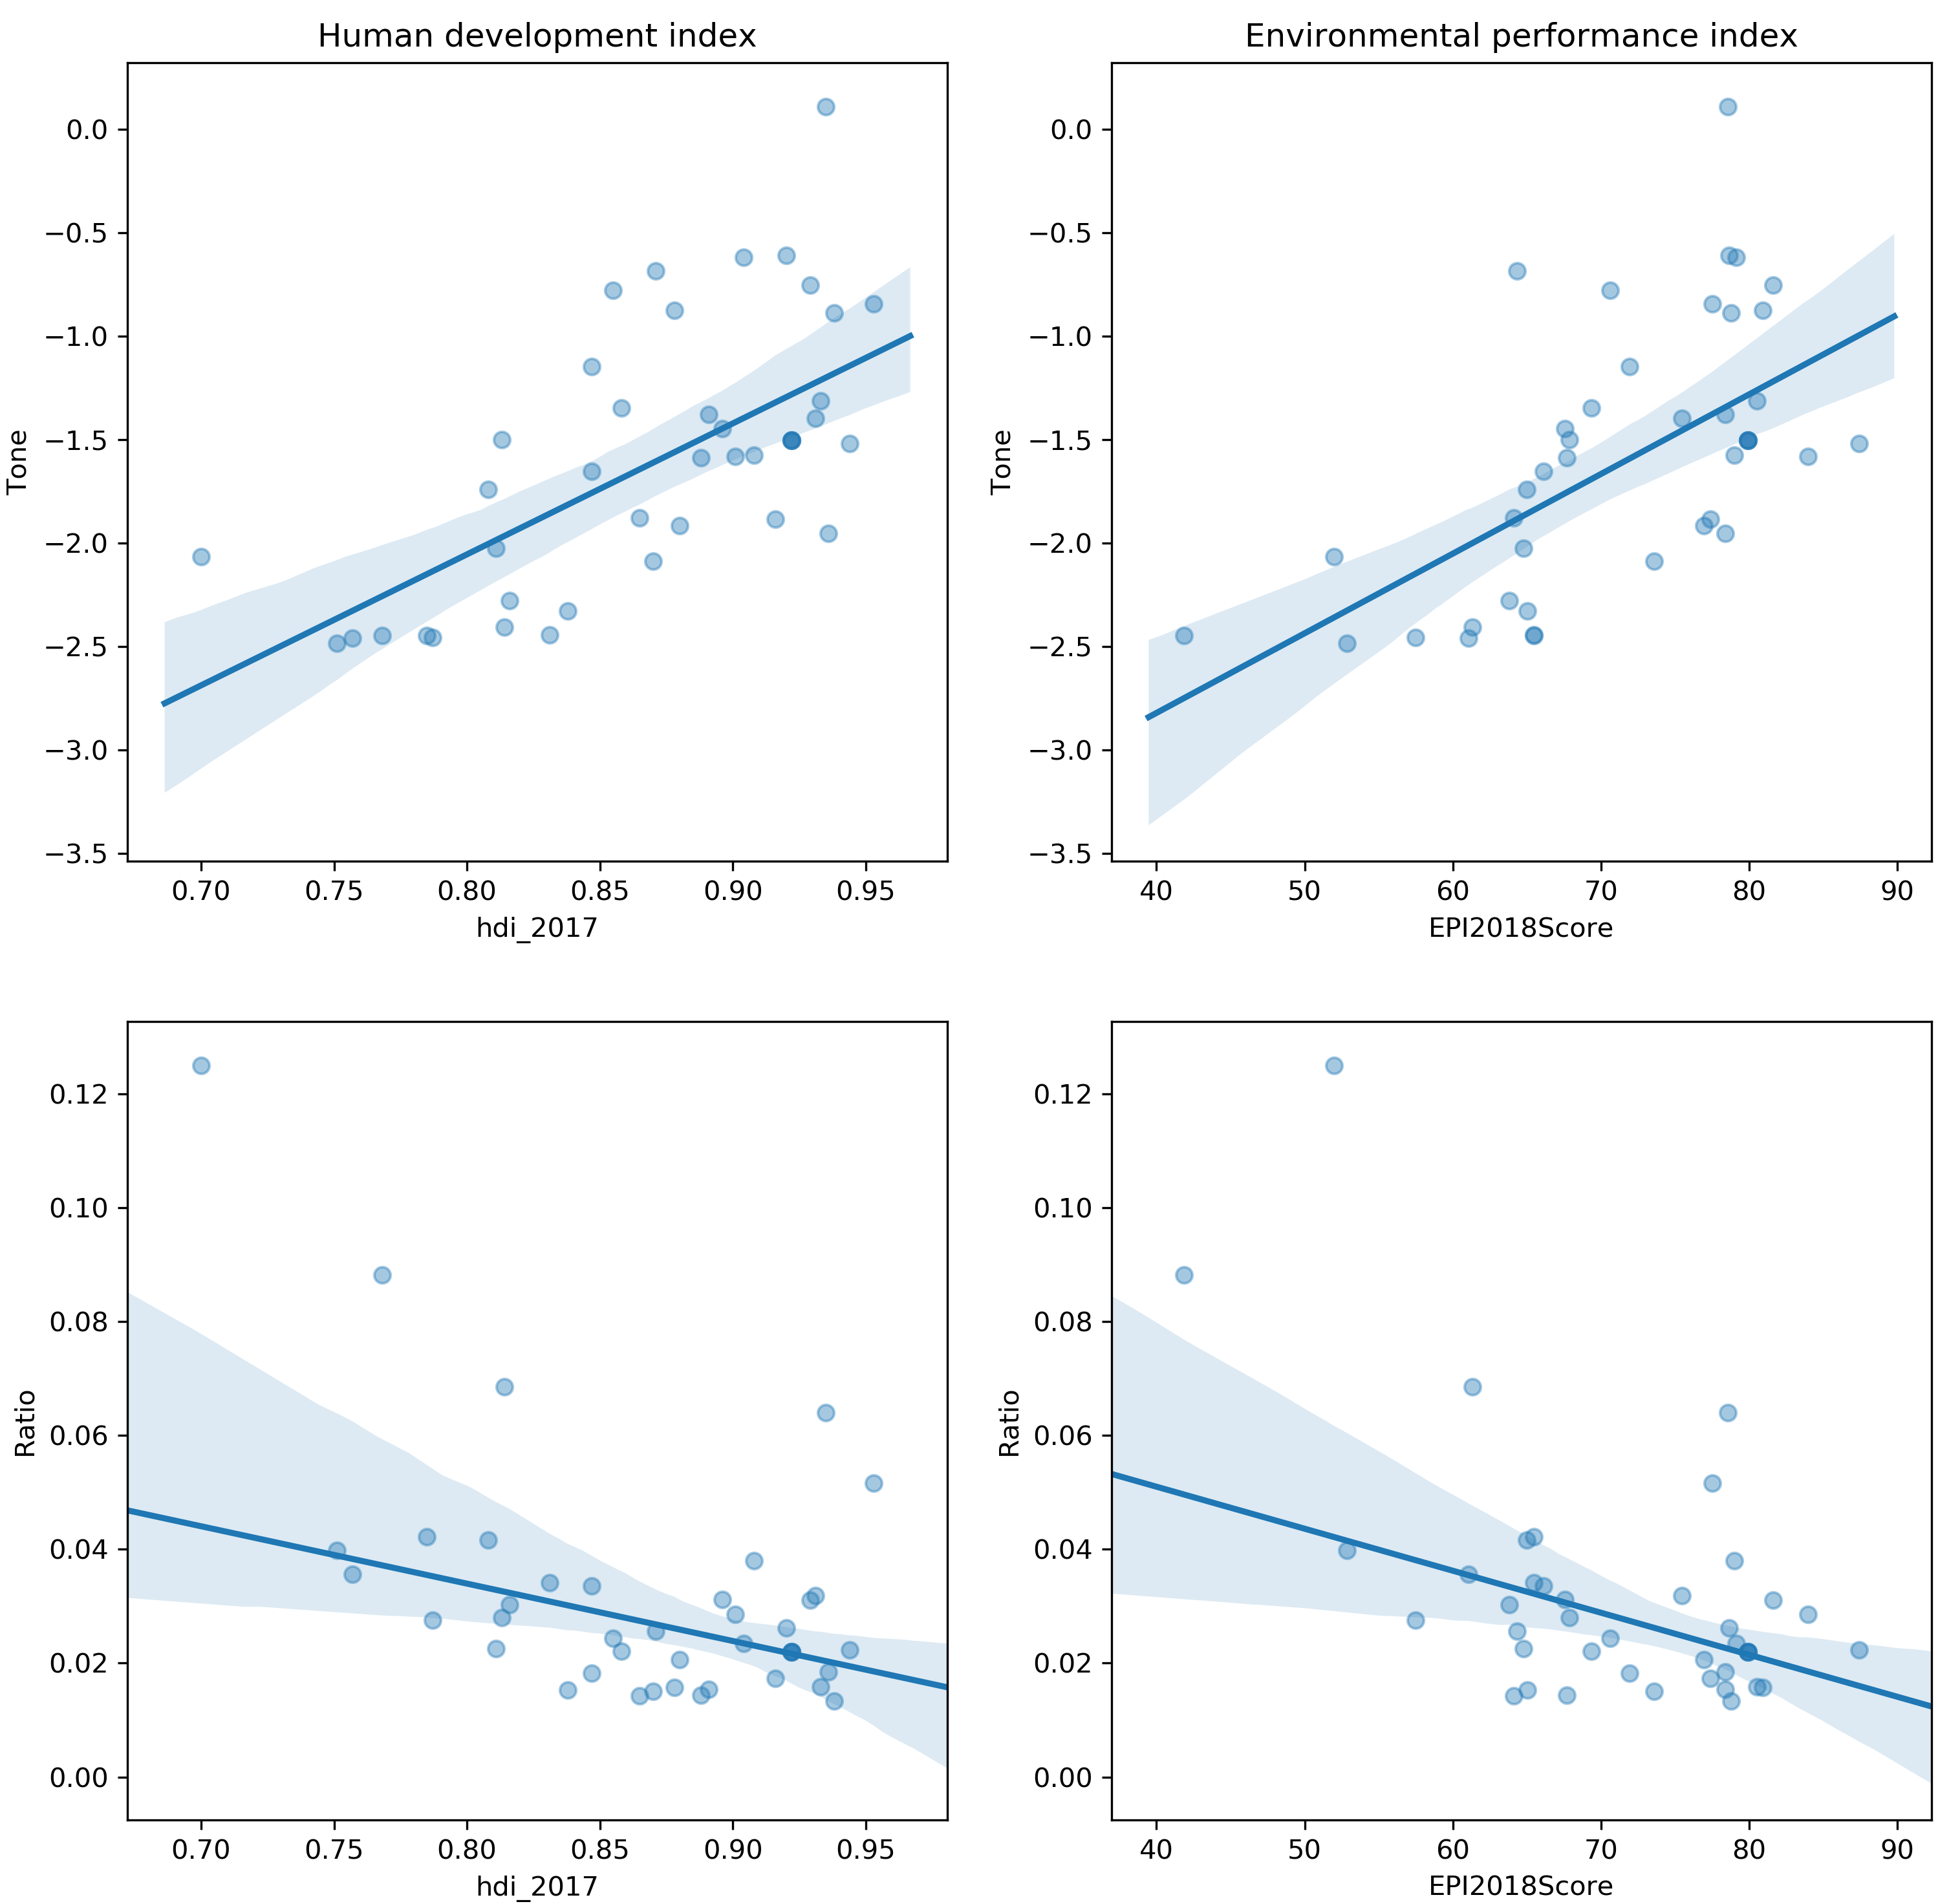
\includegraphics[scale=0.3]{corre_europe.png}
    \caption{\label{corre} Correlation with EDI and EPI of the median daily tone (top) and the median daily ratio of mentions (bottom) aggregated on European countries}
\end{figure}

We can see from figure \ref{corre} that HDI and EPI are quite correlated to the tone in articles mentioning European countries. A better developed country (high HDI/EPI) has more resource to face environmental issues and to bring concepts in favor of environments thus having a more positive median daily tone. On the contrary, the ratio of mentions is not correlated to those metrics. The tendency seem to be negative, that is countries with high HDI and EPI have a lower ratio of mentions. But this is not significant when looking at the 95\% CI or the scatter plot. This might go along the idea that we have emitted previously: the ratio of mention depends on the size of the country when regarding all the topics including environment and this metric would not be always significant to use.

\subsection{Geographical difference in point of view}
We analyze the difference in the ratio of mention for European countries when a country was mentioned by the media against when a country hosts the media. For space issue, we did not attach the Europe map showing this difference in the report, but it is present in the appendix. We now focus on two countries where there is a difference in the ratio

For the case of Germany, we can assume that the difference comes from the fact that the country gives a lot of importance to the environment. In the case of Russia, there might not be a lot of Russian media in GDELT. Moreover, among the Russian medias contained in GDELT, it is mainly about the field of fossil energies. This could make the environment over represented in media hosted by Russia in this dataset.

We cannot really conclude here. We believe that the difference could really come from the fact that the country gives more or less importance to the environment. Another reason could come from the fact that GDELT does not consider enough media from the specific country. 

\section{Conclusion}
This study investigates the news media coverage of environment events in 2015, 2016, 2017 relying on the GDELT project through the temporal and the spatial approach with the case study of European countries. We have also analyzed the majors actors involved in environmental events.

This database offers a lot of interesting information to deal with. However, to continue our analysis and to perform a better filtering, it is required to have far more time but more importantly to make use of techniques like clustering or classification.

We need to point out that GDELT is highly biased towards the United States, that is it contains far more information from the American media than other country. This need to be taken into account in all analysis done with GDELT.

\begin{thebibliography}{}
\bibitem[\protect\citename{EPI}EPI]{EPI}
Environmental Performance Index, 2018.
\\
\newblock {\url{https://epi.envirocenter.yale.edu/epi-downloads}}

\bibitem[\protect\citename{MAP}2018]{MAP}
Geographic lookup of GDELT sources
\\
\newblock{\url{https://blog.gdeltproject.org/}}
\newblock{\url{mapping-the-media-a-geographic}}
\newblock{\url{-lookup-of-gdelts-sources/}}

\bibitem[\protect\citename{GDELT}2018]{GDELT}
Global Database of Events, Language and Tone 
\\
\newblock {\url{https://www.gdeltproject.org/}}

\bibitem[\protect\citename{HDI}2018]{HDI}
Human Development Index, 2018.
\\
\newblock {\url{http://hdr.undp.org/en/content/human-development-index-hdi}}

\bibitem[\protect\citename{Louvain Method}]{Louvain Method}
{Unfolding of communities in large networks}.
\newblock 2008.
\newblock {Blondel}, V.~D. and {Guillaume}, J.-L. and {Lambiotte}, R. and {Lefebvre}, E..
\newblock {\em Journal of Statistical Mechanics: Theory and Experiment}.

\end{thebibliography}

\end{document}